\begin{frame}{Motivation}
\begin{itemize}
    \item In the near future, we'll probably have artificial agents that interact with us in the real world; meanwhile, digital agents are already a thing today.
    \item What features would we like these agents to have?
    \item Issues: Generalization, trust, interpretability, ...
    
    \item What motivated my work was the identification of three crucial factors for increased AI capability: Compositionality, communicability, and state abstraction.
\end{itemize}
\end{frame}

\note[itemize]{
    \item As the title of my thesis hints, I'm going to talk about some aspects related to intelligent agents. 
    \item Specifically, I'm going to talk about how programs, as in programming languages, might be useful representations for an agents behavior, and about my research on learning programs.
    \item Another thing I'll be talking about is the value of abstractions, more specifically how causality can help with choosing the right abstractions.
    \item So why should we care about these topics?
    
    \item AI needs to be able to deal with situations outside of those with cheap, plentiful data. Generalize to novel situations that are completely unseen.
    \item Can we trust narrow AI? When?
}

\begin{frame}{Perspective: Robot in a kitchen}
    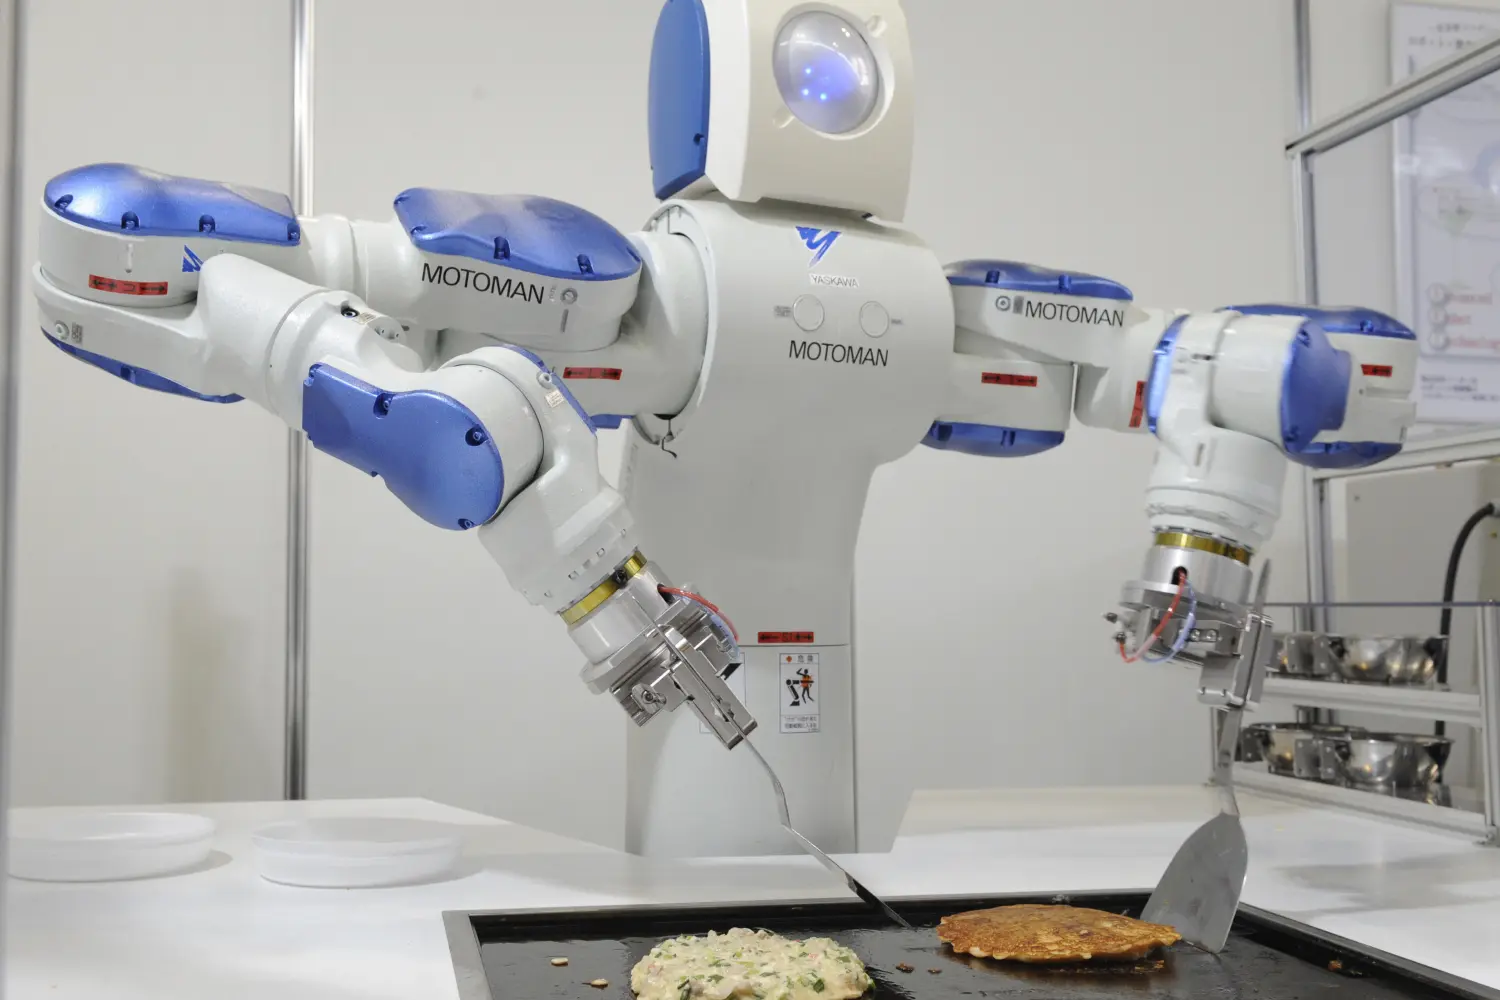
\includegraphics[width=.7\textwidth]{images/robot-cooking.png}
\end{frame}

\note[itemize]{
    \item I wanted to give you this image to consider.
    \item It relates to the 3 features I'm going to be introducing now.
    \item It's also worth thinking about during the later parts of the lecture, since it's a relatable scenario for probably everyone, yet very difficult for artificial agents.
}

\begin{frame}{1. Composition}
\begin{itemize}
    \item Behaviours are composed of other behaviours: Baking a cake involves opening a cupboard to get flour, which involves raising your arm, etc.
    \item Many behaviours are reusable: Raising your arm is not just used to open cupboards.
    \item There is never enough data to cover every case in the real world - reuse is important.
    \item Programming languages are constructed to be compositional for similar reasons, and will be one focal point in this lecture.
\end{itemize}
\end{frame}

\note[itemize]{
    \item This is the first of the 3 features. 
    \item <read slide>
}

\begin{frame}{2. Communication}
\begin{itemize}
    \item Understandable behaviours are important in many applications, such as safety critical systems.
    \item Humans might feel safer knowing how an artificial agent behaves.
    \item Beyond humans, artificial agents might benefit from communicating with each other about their behaviours; for example, in the way recipes are shared among humans.
    \item If two agents understand the same language, and share a set of grounded variables, they can share related programs.
\end{itemize}
\end{frame}

\note[itemize]{
    \item <read slide>
    \item This last point leads to the third feature, which is state abstraction.
}

\begin{frame}{3. State abstraction}
    \begin{itemize}
        \item Behaviours can be used in different settings; abstract away irrelevant aspects of states.
        \item Also related to reuse of behaviours, the same behaviours are likely applicable in similar abstract states.
        \item One way to make sense of abstraction is causality – would the outcome
(successfully cooking a meal) be any different, had the policy been to use green bowls instead of red ones?
    \end{itemize}
\end{frame}

\begin{frame}{Nethack challenge}
    %\centering
    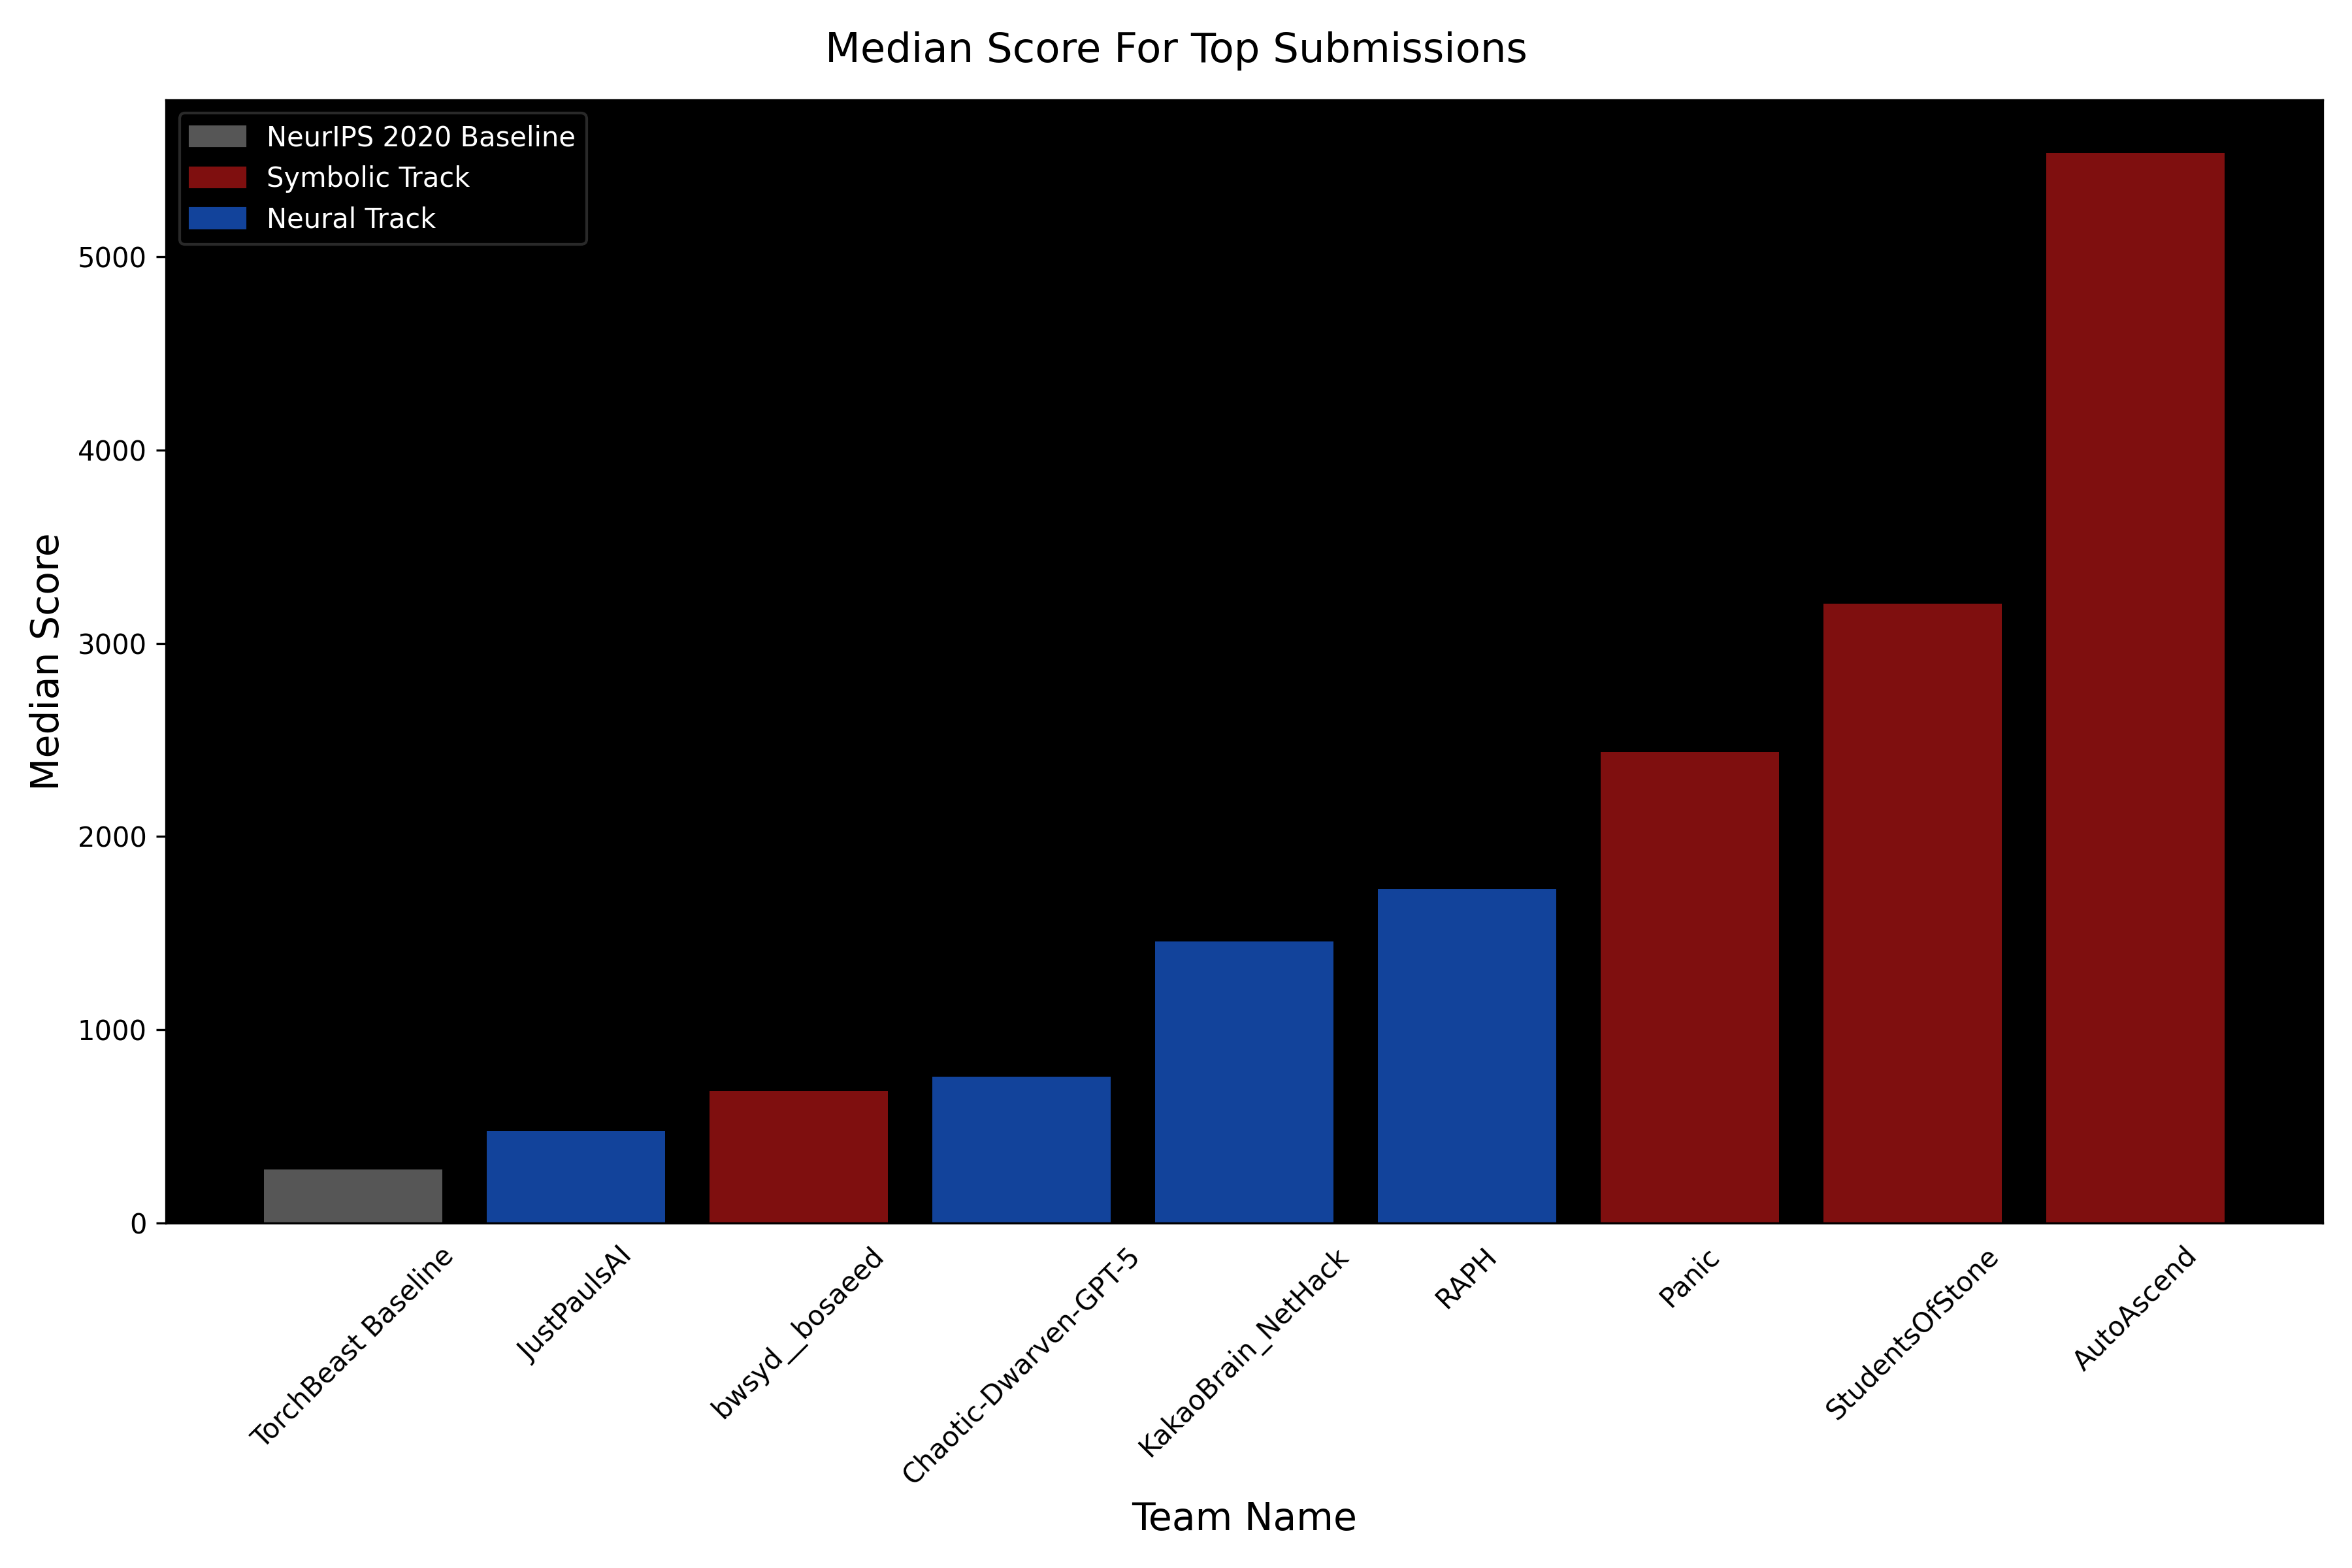
\includegraphics[width=.78\textwidth]{images/FinalScore3.png}
    \mybox{0.7, 0.55}{\fullcite{hambroInsightsNeurIPS20212022}}
\end{frame}

\note[itemize]{
    \item Challenge at NeurIPS 2021, sponsored by Facebook and Deepmind, cash prize.
    \item Roguelike game from 1987, randomly generated levels and widely considered a difficult game even for humans.
    \item Symbolic agents generally beat DL by far - best solution used a hand-coded parser to understand the scene, and hand-coded rule-based hierarchical strategies.
    \item This goes to show that explicitly represented programs are, in some sense, as of 2021 state of the art in representing policies!
    \item It also shows the value of abstraction, since the choice of high-level strategy is based on rules over human-chosen abstracted states.
    \item No agent was remotely close to "winning" the game, though.
}

\begin{frame}{Reinforcement Learning setting}
    \begin{center}
    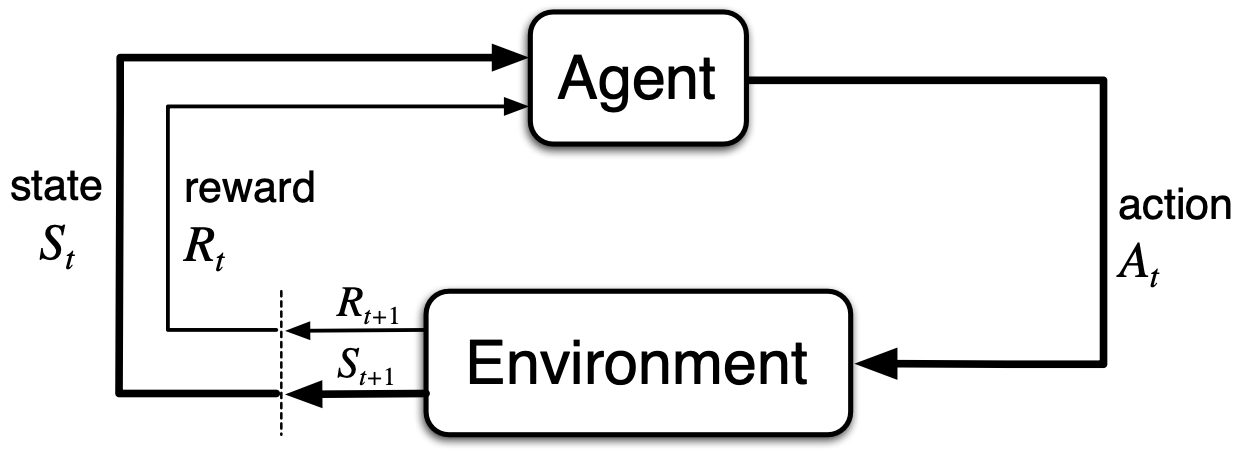
\includegraphics[width=.6\textwidth]{images/rl.png}
    \end{center}
    
    Markov Decision Process $\mathcal{M} = \{\mathcal{S}, \mathcal{A}, P, r, p_0, \gamma\}$, where $\mathcal{S}$ is the state space, $\mathcal{A}$ the action space, $P(s'|s,a)$ is the probabilistic transition function, $r(s,a)$ the reward function, $p_0$ a distribution over initial states, and $\gamma \in (0,1)$ the discount factor.
    
    The goal is to maximize the expected reward, $G_t = \sum_{i=0}^\infty \gamma^i R_{t+i+1}$. 
    
    This is achieved by the policy $\pi(s)$ that optimizes the Bellman equation:
    \begin{equation*}
        v_\pi(s) = \E_\pi\left[R_{t+1} + \gamma G_{t+1} | S_t=s\right].
    \end{equation*}
\end{frame}

\note[itemize]{
    \item 
}

\begin{frame}{Overview}
    \begin{enumerate}
        \item Programmatic policies, how to represent and learn them.
        \item State abstractions and how to learn them.
    \end{enumerate}
\end{frame}

\note[itemize]{
    \item
}